\documentclass[11pt]{article}
\usepackage[utf8]{inputenc}
\usepackage[T1]{fontenc}
\usepackage{amsmath,amssymb}
\usepackage{geometry}
\usepackage{listings}
\usepackage{xcolor}
\usepackage{hyperref}
\usepackage{tikz}
\usepackage{booktabs}
\usepackage{enumitem}
\usetikzlibrary{calc, arrows.meta, positioning, shapes.geometric, fit, decorations.pathreplacing}

\geometry{margin=2.2cm}

\lstdefinelanguage{Rust}{
  keywords={fn,let,mut,for,in,if,else,while,loop,match,return,struct,impl,pub,use,mod,as,where,move,ref,self,Self,crate,super,async,await,unsafe,const,static,type,enum,trait,dyn,true,false,continue,break},
  keywordstyle=\color{blue!70!black}\bfseries,
  ndkeywords={Vec,Vec3,Mat4,Mesh,MeshVertex,SceneNode,Scene,PbrMaterial,TreeParams,u32,usize,f32,f64,bool,Option,Some,None,Result,Ok,Err,String,Morphology,Tree,k,PI},
  ndkeywordstyle=\color{purple!70!black}\bfseries,
  sensitive=true,
  comment=[l]{//},
  morecomment=[s]{/*}{*/},
  commentstyle=\color{green!50!black}\itshape,
  stringstyle=\color{red!70!black},
  morestring=[b]",
}

\lstset{
  basicstyle=\ttfamily\footnotesize,
  breaklines=true,
  frame=single,
  language=Rust,
  showstringspaces=false,
  tabsize=2,
}

\title{TPMS Shell and Skeletal Morphology Generation\\in engvis}
\author{engvis}
\date{\today}

\begin{document}
\maketitle

\begin{abstract}
Triply Periodic Minimal Surfaces (TPMS) can be used in three distinct
morphology modes for engineering applications: \emph{minimal surface}
(the classic open sheet $f=0$), \emph{shell} (a thick-walled hollow
structure $g = \max(f-\delta,\;-f-\delta) = |f|-\delta$), and
\emph{skeletal} (a solid strut network $f - C = 0$).  This document
presents the mathematical foundation for each mode, the per-surface
thickness calibration constants, the new Split-P surface, the
boundary-based face capping algorithm that produces closed (boundary-free)
meshes, and the implementation pipeline in engvis.
\end{abstract}

% =====================================================================
\section{TPMS Morphology Types}

A triply periodic minimal surface is defined as the zero level-set of
a smooth function $f\colon\mathbb{R}^3 \to \mathbb{R}$:
\begin{equation}\label{eq:tpms-levelset}
  \mathcal{S} = \bigl\{\mathbf{x} \in \mathbb{R}^3 \;\big|\; f(\mathbf{x}) = 0\bigr\}.
\end{equation}
This open surface divides space into two regions ($f>0$ and $f<0$).
Depending on the engineering application, three morphology modes are
useful (see Figure~\ref{fig:morphology-comparison}).

\begin{figure}[h]
\centering
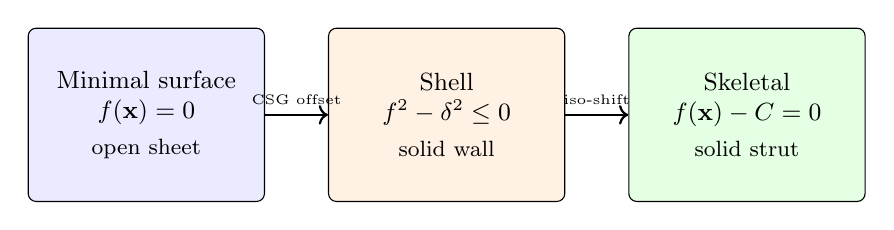
\begin{tikzpicture}[
    every node/.style={font=\small},
    box/.style={draw, minimum width=30mm, minimum height=22mm,
                rounded corners=1mm, align=center},
  ]
  \node[box, fill=blue!8]  (min) {Minimal surface\\$f(\mathbf{x})=0$\\[2pt]\footnotesize open sheet};
  \node[box, fill=orange!10, right=8mm of min] (shell)
    {Shell\\$f^2-\delta^2\le 0$\\[2pt]\footnotesize solid wall};
  \node[box, fill=green!10, right=8mm of shell] (skel)
    {Skeletal\\$f(\mathbf{x})-C=0$\\[2pt]\footnotesize solid strut};

  \draw[->, thick] (min) -- node[above, font=\tiny]{CSG offset} (shell);
  \draw[->, thick] (shell) -- node[above, font=\tiny]{iso-shift} (skel);
\end{tikzpicture}
\caption{Three TPMS morphology modes: minimal surface (open sheet),
shell (two offset surfaces forming a hollow wall), and skeletal
(shifted iso-level forming a solid strut network).}
\label{fig:morphology-comparison}
\end{figure}

\subsection{Minimal Surface Mode}

The default mode extracts the zero level-set directly:
\begin{equation}
  g(\mathbf{x}) = f(\mathbf{x}).
\end{equation}
This produces a thin, open surface---the classic TPMS sheet.  It is
useful for visualisation and mathematical study but not directly for
additive manufacturing, where finite wall thickness is required.

\subsection{Shell Mode}\label{sec:shell}

Shell mode produces a \emph{thick-walled solid structure}: a thin
band of material straddling the minimal surface $f=0$, bounded by the
two offset iso-surfaces $f = \pm\delta$.  The solid wall region is the
sub-level set
\begin{equation}\label{eq:shell}
  \mathcal{S}_{\text{shell}}
    = \bigl\{\,\mathbf{x} : f(\mathbf{x})^2 - \delta^2 \le 0 \,\bigr\}
    = \bigl\{\,\mathbf{x} : |f(\mathbf{x})| \le \delta \,\bigr\},
\end{equation}
described by the \textbf{smooth} field $g = f^2 - \delta^2$, which is
negative \emph{inside} the wall and positive outside.

\paragraph{Geometric thickness normalisation.}
The user-facing parameter $t$ is a \emph{geometric} wall thickness
(the physical distance across the wall), not a field offset.  Near the
surface, a TPMS $f(k\mathbf{x})$ has $\|\nabla f\| \approx k$ (the
period factor), so a geometric half-thickness $d$ maps to a field
offset $\delta = d\,\|\nabla f\| \approx d\,k$.  engvis therefore
sets
\begin{equation}\label{eq:thickness}
  \delta = \tfrac{1}{2}\, t \, k,
  \qquad k = \text{tpms\_period},
\end{equation}
so that the meshed wall has true geometric thickness $\approx t$.  For
non-TPMS surfaces, $\|\nabla f\| \approx 1$ and $k$ falls back to $1$.

\paragraph{Why $f^2-\delta^2$, not $|f|-\delta$.}
Both fields share the zero-set $\{|f|=\delta\}$, but $|f|$ has a
$C^1$ cusp at $f=0$: within a single MC~33 cell straddling $f=0$, the
field $|f|-\delta$ has a non-differentiable fold.  The squared field
$f^2-\delta^2$ is smooth everywhere, so MC~33's linear interpolation
stitches adjacent cells without artefacts---\emph{provided the cell
size is smaller than the wall thickness}.

\paragraph{Resolution requirement.}
Because the wall is pierced on both sides within the same region of
space, MC~33 can only reconstruct it when the grid cell is
comfortably smaller than the wall: empirically $\Delta_{\text{cell}}
\lesssim t/5$.  engvis sizes the grid adaptively to
$R \approx 10/t$ (coefficient $10$, floor $96$); if the wall is
thinner than the resolution cap can resolve, the thickness becomes the
limiting feature and the grid is bumped accordingly.

\begin{table}[h]
\centering
\caption{Shell mesh topology for gyroid at geometric thickness
$t=0.1$ ($k=4 \Rightarrow \delta=0.2$).  Once the cell size drops
below the wall thickness ($R\ge 96$), the mesh is a single watertight
closed solid.}
\label{tab:shell-fragments}
\begin{tabular}{lccccc}
\toprule
Field & $R$ & $\chi$ & components & boundary edges & watertight \\
\midrule
$f^2-\delta^2$ & 64  & $-53$ & 9 & 82 & no  \\
$f^2-\delta^2$ & 96  & $-38$ & \textbf{1} & \textbf{0} & \textbf{yes} \\
$f^2-\delta^2$ & 128 & $-38$ & \textbf{1} & \textbf{0} & \textbf{yes} \\
\bottomrule
\end{tabular}
\end{table}

\paragraph{Closed solid via box-CSG.}
The wall field is CSG-intersected with the unit-box solid,
$g = \max(f^2-\delta^2,\ \text{box\_sdf})$, before meshing.  Marching
Cubes then generates cap faces on $x/y/z = \pm 1$ itself, yielding a
single watertight closed solid with \emph{zero boundary edges}.  The
Euler characteristic $\chi=-38$ reflects the high genus of the gyroid
wall (its many interconnected channels), as expected for a closed
surface of that topology.

\paragraph{Gradient and normals.}
The wall surface $\{f^2=\delta^2\}$ has gradient
$\nabla(f^2-\delta^2) = 2f\,\nabla f$, which is non-degenerate on the
surface itself (where $|f|=\delta\neq 0$).  engvis overwrites vertex
normals with this analytic gradient, producing correct two-sided
lighting.

\subsection{Skeletal Mode}\label{sec:skeletal}

Skeletal mode produces a \emph{solid strut network} by shifting the
iso-level of the TPMS function:
\begin{equation}\label{eq:skeletal}
  g(\mathbf{x}) = f(\mathbf{x}) - C,
\end{equation}
where $C$ is the iso-level offset parameter.

\paragraph{Effect of $C$.}
When $C = 0$, this reduces to the minimal surface mode.  As $C$
increases, the region $\{g \le 0\} = \{f \le C\}$ expands, filling
more of the unit cell with ``solid'' material.  The resulting surface
$f = C$ is topologically distinct from the minimal surface: instead of
an open sheet, it forms a connected network of solid struts along the
edges and vertices of the TPMS unit cell.

The gradient is simply $\nabla g = \nabla f$, so surface normals are
unaffected by the shift---a desirable property.

\paragraph{Negative $C$.}
When $C < 0$, the solid region shrinks and the void region expands.
This produces the \emph{complementary} structure: thin channels
instead of thick struts.

% =====================================================================
\section{Thickness Calibration}\label{sec:calibration}

The user-facing thickness $t$ is a true \emph{geometric} wall
thickness.  To realise it consistently across surfaces, engvis
converts $t$ into a field offset $\delta$ using the gradient magnitude
of the implicit function near its zero-set (Eq.~\ref{eq:thickness}):
\begin{equation}
  \delta = \tfrac{1}{2}\, t \, \|\nabla f\|,
  \qquad \|\nabla f\| \approx k = \text{tpms\_period}.
\end{equation}

For a TPMS evaluated as $f(k\mathbf{x})$, the chain rule gives
$\|\nabla_{\mathbf{x}} f\| = k\,\|\nabla_{\mathbf{u}} \hat f\|$, and
the dimensionless gradient $\|\nabla_{\mathbf{u}}\hat f\|$ is $O(1)$
on the surface for all the standard TPMS types
(Table~\ref{tab:calibration}).  Using $k$ as a first-order estimate
therefore yields a wall whose geometric thickness is within a few
percent of $t$---accurate enough for visualisation and consistent
across surfaces without per-surface tuning.

\begin{table}[h]
\centering
\caption{Dimensionless surface-gradient magnitude
$\|\nabla_{\mathbf{u}}\hat f\|$ near the zero-set (the residual
correction absorbed by the $k$ estimate).}
\label{tab:calibration}
\begin{tabular}{lcc}
\toprule
\textbf{Surface} & $\|\nabla_{\mathbf{u}}\hat f\|$ & \textbf{Notes} \\
\midrule
Gyroid           & $\approx 1.2$ & three-term product \\
Schwarz D        & $\approx 1.3$ & four-term sum \\
Schwarz P        & $\approx 1.0$ & simple cosine sum \\
Schoen IWP       & $\approx 1.1$ & \\
Neovius          & $\approx 1.2$ & \\
\bottomrule
\end{tabular}
\end{table}

Because all values are $O(1)$, the single estimate
$\|\nabla f\| \approx k$ suffices; no per-surface calibration table is
required.

% =====================================================================
\section{Split-P Surface}\label{sec:split-p}

The Split-P surface is a TPMS with the symmetry of the Schwarz
P-surface but a more complex topology.  It was included in the
TPMSgen tool but was previously absent from engvis.  Its implicit
equation is:
\begin{equation}\label{eq:split-p}
\begin{aligned}
  f_{\text{Split-P}}(\mathbf{x}) &=
    1.1\bigl[\sin(2kx)\cos(ky)\sin(kz)
           + \sin(kx)\sin(2ky)\cos(kz)
           + \cos(kx)\sin(ky)\sin(2kz)\bigr] \\
  &\quad - 0.2\bigl[\cos(2kx)\cos(2ky)
                   + \cos(2ky)\cos(2kz)
                   + \cos(2kz)\cos(2kx)\bigr] \\
  &\quad - 0.4\bigl[\cos(2kx) + \cos(2ky) + \cos(2kz)\bigr].
\end{aligned}
\end{equation}

Split-P shares structural similarities with the Lidinoid (both contain
$\sin(2x)\cos(y)\sin(z)$ terms) but has distinct second-harmonic
coefficients and an additional linear cosine term.  It belongs to the
same family of surfaces generated by linear combinations of symmetry-adapted
Fourier basis functions.

% =====================================================================
\section{Complete Surface Catalogue}

Table~\ref{tab:catalogue} lists all eleven TPMS surfaces supported by
engvis with their implicit equations $f(\mathbf{x}) = 0$, where
$\mathbf{x} = (kx, ky, kz)$ and $k = 2\pi/\lambda$ is the wave number
controlled by the Period slider.

\begin{table}[h]
\centering
\caption{TPMS surface catalogue in engvis.}
\label{tab:catalogue}
\small
\begin{tabular}{lp{9cm}}
\toprule
\textbf{Name} & \textbf{Implicit equation $f = 0$} \\
\midrule
Gyroid & $\sin x\cos y + \sin y\cos z + \sin z\cos x$ \\
Schwarz P & $\cos x + \cos y + \cos z$ \\
Schwarz D & $\sin x\sin y\sin z + \sin x\cos y\cos z + \cos x\sin y\cos z + \cos x\cos y\sin z$ \\
Schoen IWP & $2(\cos x\cos y + \cos y\cos z + \cos z\cos x) - (\cos 2x + \cos 2y + \cos 2z)$ \\
Neovius & $3(\cos x + \cos y + \cos z) + 4\cos x\cos y\cos z$ \\
F-RD & $4\cos x\cos y\cos z - (\cos 2x\cos 2y + \cos 2y\cos 2z + \cos 2z\cos 2x)$ \\
Lidinoid & $\tfrac{1}{2}[\sin 2x\cos y\sin z + \sin x\sin 2y\cos z + \cos x\sin y\sin 2z]
            - \tfrac{1}{2}[\cos 2x\cos 2y + \cos 2y\cos 2z + \cos 2z\cos 2x] + 0.15$ \\
Split-P & see Eq.~\eqref{eq:split-p} \\
Fischer-Koch S & $\cos 2x\sin y\cos z + \cos 2y\sin z\cos x + \cos 2z\sin x\cos y$ \\
Fischer-Koch Y & $2\cos x\cos y\cos z + \sin 2x\sin y + \sin 2y\sin z + \sin 2z\sin x$ \\
Fischer-Koch CP & $\cos x + \cos y + \cos z + 4\cos x\cos y\cos z$ \\
\bottomrule
\end{tabular}
\end{table}

% =====================================================================
\section{Implementation Pipeline}

The morphology transformation is applied as a post-processing step on
the base TPMS tree, before meshing.  Figure~\ref{fig:pipeline} shows
the complete data flow.

\begin{figure}[h]
\centering
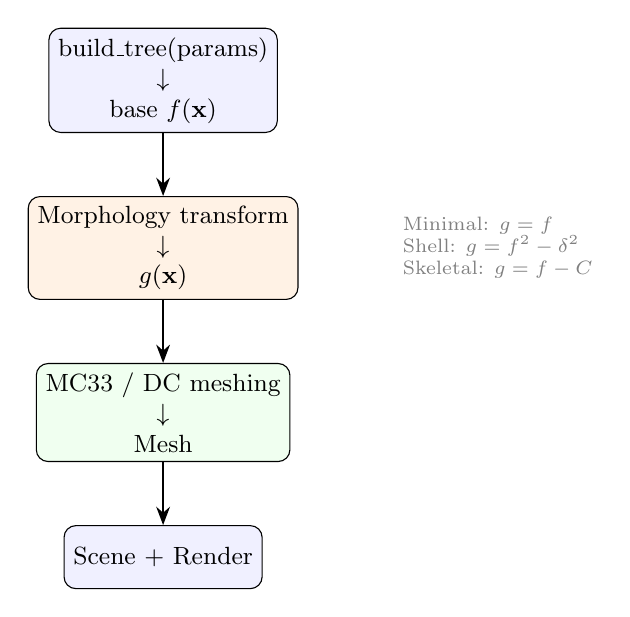
\begin{tikzpicture}[
    every node/.style={font=\small},
    block/.style={draw, rounded corners=1.5mm, minimum height=8mm,
                  align=center, fill=blue!6},
    morph/.style={draw, rounded corners=1.5mm, minimum height=8mm,
                  align=center, fill=orange!10},
    mesh/.style={draw, rounded corners=1.5mm, minimum height=8mm,
                 align=center, fill=green!6},
    arr/.style={->, thick, >=Stealth},
  ]

  \node[block] (tree) {build\_tree(params)\\$\downarrow$\\base $f(\mathbf{x})$};
  \node[morph, below=8mm of tree] (morph) {Morphology transform\\$\downarrow$\\$g(\mathbf{x})$};
  \node[mesh, below=8mm of morph] (mc) {MC33 / DC meshing\\$\downarrow$\\Mesh};
  \node[block, below=8mm of mc] (scene) {Scene + Render};

  \draw[arr] (tree) -- (morph);
  \draw[arr] (morph) -- (mc);
  \draw[arr] (mc) -- (scene);

  % Side annotations
  \node[right=12mm of morph, font=\scriptsize, text=gray, align=left]
    {Minimal: $g = f$\\Shell: $g = f^2-\delta^2$\\Skeletal: $g = f - C$};
\end{tikzpicture}
\caption{Data flow for TPMS morphology generation.  The base TPMS
function $f$ is first constructed by \texttt{build\_tree}, then
transformed by the morphology module into $g$, and finally meshed by
the standard MC33 or DC pipeline.}
\label{fig:pipeline}
\end{figure}

\subsection{Code Structure}

The morphology transformation is implemented in \texttt{build\_scene}.
For minimal surface and skeletal modes, the tree is transformed
algebraically and passed to the standard \texttt{build\_mesh}
pipeline.  For shell mode, the original tree is passed to
\texttt{build\_shell\_mesh}, which meshes the smooth wall solid
$f^2-\delta^2$:

\begin{lstlisting}
// build_scene: geometric thickness -> field offset
let k = self.tpms_period.max(1.0);     // |grad f| ~ k
let shell_half_t = 0.5 * thickness * k; // delta

let tree = match self.morphology {
    MinimalSurface | Shell => tree,    // Shell handled below
    Skeletal => tree - iso_level,
};

let mesh = if matches!(self.morphology, Morphology::Shell) {
    // Smooth wall solid f^2 - delta^2, box-CSG, single MC33 pass.
    build_shell_mesh(
        tree.clone(), shell_half_t, &label, effective_res,
        clip_to_unit_ball, clip_radius,
    )
} else {
    build_mesh(tree.clone(), &label, ...)
};
\end{lstlisting}

\begin{lstlisting}
// build_shell_mesh: smooth wall solid + box-CSG, single pass
fn build_shell_mesh(tree, half_t, name, res, ...) -> Mesh {
    // Box-CSG: intersect with unit-box solid so MC caps the faces.
    let box_sdf = |x|.max(|y|).max(|z|) - c;

    // Thin-wall solid: g = f^2 - half_t^2 (smooth, no cusp).
    let wall  = tree.square() - half_t * half_t;
    let field = wall.max(box_sdf);
    build_mc33_mesh_domain(field, name, res, false, half)
}
\end{lstlisting}

The Fidget implicit modelling library represents the expression as a
computational tree (\texttt{Tree}) with overloaded arithmetic
operators: \texttt{tree.square()} builds $f^2$, and \texttt{.max()}
performs the CSG intersection with the box solid.  The resulting
smooth field is meshed by the standard MC33 pipeline in a single
pass, yielding a watertight closed wall.

\subsection{Interaction with Meshing}

Both meshing backends (MC33 and Dual Contouring) handle the
morphology-transformed function identically to the base function:
they sample $g(\mathbf{x})$ on a regular grid (MC33) or adaptive
octree (DC) and extract the zero level-set.

For \textbf{shell mode}, the smooth field $g = f^2-\delta^2$ is
CSG-intersected with the unit-box solid
($\max(g,\ \text{box\_sdf})$), so MC33 generates cap faces on
$x/y/z = \pm 1$, producing a closed solid with zero boundary edges.
Because $f^2$ is smooth (no $C^1$ cusp), MC33's linear interpolation
stitches adjacent cells cleanly once the cell size is below the wall
thickness ($\Delta_{\text{cell}} \lesssim t/5$); below that the wall
fragments (Table~\ref{tab:shell-fragments}, $R=64$).  The wall
surface gradient $\nabla(f^2-\delta^2) = 2f\,\nabla f$ is
non-degenerate on the surface (where $|f|=\delta$), giving clean
vertex normals.

For \textbf{skeletal mode}, the function $g = f - C$ has the same
gradient structure as the base TPMS ($\nabla g = \nabla f$), so both
backends produce clean results.  The skeletal mesh is a closed solid
(box-CSG), so it uses the boundary capping described in
Section~\ref{sec:capping}.

\subsection{Box-Face Capping via Boundary Loops}\label{sec:capping}

Shell and skeletal modes define a \emph{solid region}
($g \le 0$) bounded by the iso-surface and the domain boundary.
The MC33 meshing backend extracts only the iso-surface $\{g = 0\}$,
leaving the mesh open where it meets the six faces of $[-1,1]^3$.
To produce a closed volume, engvis identifies the \emph{MC33 boundary
edges} on the box surface and fan-triangulates the enclosed loops
directly---reusing the existing boundary vertices so that cap and body
share the same vertex indices (Figure~\ref{fig:capping}).

\emph{Note:} Shell mode uses the same box-CSG capping mechanism
(via \texttt{build\_mc33\_mesh\_domain}), applied independently to
each of the two iso-surfaces.  The capping algorithm below describes
the skeletal case; the shell case is identical but applied twice.

\begin{figure}[h]
\centering
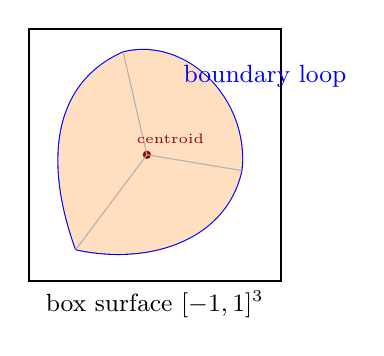
\begin{tikzpicture}[
    every node/.style={font=\small},
    arr/.style={->, thick, >=Stealth},
  ]
  % Box face with contour
  \draw[thick] (0,0) rectangle (3.2,3.2);

  % g=0 contour (closed loop)
  \draw[blue, thick] (0.6,0.4) .. controls (0.2,1.5) and (0.3,2.5) .. (1.2,2.9)
    .. controls (2.0,3.1) and (2.8,2.3) .. (2.7,1.4)
    .. controls (2.5,0.5) and (1.5,0.2) .. (0.6,0.4);

  % Centroid and fan lines
  \coordinate (C) at (1.5,1.6);
  \fill[orange!25] (0.6,0.4) .. controls (0.2,1.5) and (0.3,2.5) .. (1.2,2.9)
    .. controls (2.0,3.1) and (2.8,2.3) .. (2.7,1.4)
    .. controls (2.5,0.5) and (1.5,0.2) .. (0.6,0.4);
  \fill[red!60!black] (C) circle (1.5pt);
  \draw[gray!60] (C) -- (0.6,0.4);
  \draw[gray!60] (C) -- (1.2,2.9);
  \draw[gray!60] (C) -- (2.7,1.4);

  % Labels
  \node at (1.6,-0.3) {box surface $[-1,1]^3$};
  \node[blue] at (3.0,2.6) {boundary loop};
  \node[red!60!black] at (1.8,1.8) {\tiny centroid};
\end{tikzpicture}
\caption{Boundary-based face capping: the MC33 boundary edges
(blue) on the box surface are chained into closed loops, then
fan-triangulated from their centroid (red dot) to produce cap
triangles (orange) that close the volume.  Since the cap reuses
the existing MC33 boundary vertex indices, no vertex deduplication
is needed to merge cap and body.}
\label{fig:capping}
\end{figure}

\paragraph{Prerequisites.}
The algorithm requires that all MC33 boundary edges lie on the
surface of $[-1,1]^3$ (no \emph{interior} boundary edges).  For the
CSG shell formula $g = |f| - \delta$, this holds at MC33 resolution
$\ge 96$.  At resolution 64, the old squared formula produced 19
spurious micro-components with $\sim$1500 interior boundary edges
that could not be capped.  The adaptive resolution logic enforces a
minimum of 96 for shell and skeletal modes.

\paragraph{Algorithm.}
\begin{enumerate}[leftmargin=2em]
  \item \textbf{Identify boundary edges}: an edge shared by exactly
    one triangle.  Classify each as \emph{surface} (both endpoints on
    the box surface, $|x_i| > 1 - \varepsilon$) or \emph{interior}.
    If any interior boundary edges exist, abort capping.
  \item \textbf{Build adjacency graph}: vertex $\to$ list of
    neighbouring boundary vertices.  Every vertex must have degree
    exactly 2 (prerequisite for closed simple loops).
  \item \textbf{Chain into closed loops}: greedy traversal from an
    arbitrary unvisited vertex, following unvisited neighbours until
    the loop closes.  Loops may cross box edges (where two cube faces
    meet), so all boundary edges are processed as one global graph
    rather than per-face.
  \item \textbf{Fan-triangulate each loop}: add a centroid vertex
    $\mathbf{c} = \frac{1}{n}\sum \mathbf{v}_i$ and create triangles
    $(\mathbf{c}, \mathbf{v}_i, \mathbf{v}_{i+1})$.  The loop normal
    is estimated via Newell's method:
    \begin{equation}
      \mathbf{n} = \sum_{i=0}^{n-1} (\mathbf{v}_i - \mathbf{v}_{i+1})
                   \times (\mathbf{v}_i + \mathbf{v}_{i+1}),
    \end{equation}
    which handles non-planar loops.  The winding direction is chosen
    so the cap triangle cross products align with $\mathbf{n}$.
  \item \textbf{Signed-volume check}: compute
    $V = \sum_{\triangle} \mathbf{p}_0 \cdot (\mathbf{p}_1 \times \mathbf{p}_2)$.
    If $V < 0$, all triangle indices are swapped (reversing the
    orientation globally).
\end{enumerate}

\paragraph{Why reusing MC33 vertices matters.}
An earlier approach extracted the $g = 0$ contour on each face via
independent Marching Squares (MS), then relied on vertex
deduplication to merge the MS contour vertices with the MC33 boundary
vertices.  Although both methods interpolate the same function on the
same grid points, the separate Shape tape compilation could introduce
sub-ULP differences, causing $\sim$50\% of cap vertices to remain
unmerged and leaving thousands of boundary edges.

The direct boundary approach eliminates this entirely: the cap
triangles reference the \emph{same vertex indices} as the MC33 body,
so no merging is needed.  The only new vertices are the loop
centroids.

\paragraph{Topology verification.}
After capping, the mesh topology is verified via the Euler
characteristic $\chi = V - E + F$ and the boundary edge count.
For the Gyroid shell (period $k=4$, thickness $t=1.0$):
\begin{itemize}[leftmargin=2em]
  \item \emph{Before capping}: $\chi = -20$, 4 components,
    5232 boundary edges (all on box faces), 0 interior boundaries.
  \item \emph{After capping}: $\chi = 0$, 4 components,
    \textbf{0 boundary edges}, 0 non-manifold edges.
\end{itemize}
The 4 components correspond to the two offset surfaces ($f = \pm\delta$)
of the two interpenetrating Gyroid channel networks---a topologically
correct result.  Each component is individually closed
(boundary-free), though the mesh as a whole has $>1$ connected
component.

% =====================================================================
\section{Comparison with TPMSgen}

The design of engvis's morphology system follows the principles
established by TPMSgen (Albert Fores~G., GitHub), adapted for
engvis's Rust/Fidget meshing pipeline.  Key differences are summarised
in Table~\ref{tab:comparison}.

\begin{table}[h]
\centering
\caption{Comparison of TPMSgen and engvis TPMS generation.}
\label{tab:comparison}
\begin{tabular}{lp{4.5cm}p{4.5cm}}
\toprule
\textbf{Feature} & \textbf{TPMSgen} & \textbf{engvis} \\
\midrule
Shell generation & Two MC passes at $\pm\delta$, concat meshes & CSG $\max(f-\delta,\,-f-\delta)$ single pass \\
Skeletal generation & MC at $f=0$, boolean diff with box & MC at $f=C$, box clip \\
Boolean operations & Blender engine (trimesh) & CSG $\max/\min$ on expression tree \\
Meshing backend & skimage marching\_cubes & Custom MC33 + Fidget DC \\
Watertight closure & Iterative padding + hole filling & Boundary-loop fan capping \\
Surface count & 10 (5 shell + 5 skeletal) & 11 (all in all modes) \\
Normal handling & pyvista flip normals & Gradient overwrite + signed-volume check \\
\bottomrule
\end{tabular}
\end{table}

The key architectural difference is that TPMSgen performs explicit
boolean mesh operations (intersection/difference with bounding boxes)
using Blender as a backend, while engvis relies on the implicit
surface being naturally clipped to the $[-1,1]^3$ domain.  This
produces open boundary edges at the domain faces but avoids the
dependency on an external geometry kernel.

% =====================================================================
\section{Usage}

In the engvis UI, morphology controls appear in the \textbf{Source}
panel when a TPMS surface is selected:

\begin{enumerate}[leftmargin=2em]
  \item Select a TPMS surface from the dropdown (e.g.\ Gyroid).
  \item Adjust the \textbf{Period k} slider to set the spatial frequency.
  \item Choose a morphology mode:
    \begin{itemize}
      \item \textbf{Minimal surface} ($f=0$) --- open sheet.
      \item \textbf{Shell} ($|f|-\delta=0$) --- adjust \textbf{Thickness}.
      \item \textbf{Skeletal} ($f-C=0$) --- adjust \textbf{C value}.
    \end{itemize}
  \item Click \textbf{Re-mesh} to rebuild the surface.
\end{enumerate}

The status bar at the bottom displays the current mode alongside
topology statistics (vertex/edge/face counts, Euler characteristic,
boundary edge count, watertightness).

\end{document}
